\documentclass{ijsra}
\def\IJSRAidentifier{\currfilebase} %<---- don’t change this!
\def\submission{}%YYYY-MM-DD
\def\acceptance{}%YYYY-MM-DD
%-------Title | Email | Keywords | Abstract-------------
\def\shorttitle{ESHE Meeting Review}
\def\maintitle{Review of the European Society for the Study of Human Evolution – 7\textsuperscript{th} Annual Meeting, September 21\textsuperscript{st} - 23\textsuperscript{rd} 2017 Leiden, The Netherlands}
\def\cmail{gonzlinares@gmail.com}
\def\keywords{NO KEYWORDS}
%\def\keywordname{}%<--- redefine the name “Keywords“ in needed language
%\def\abstract{}
%--------Author’s names------------
\def\authorone{Gonzalo Linares Matás}
%-------Biographical information-------------
\def\bioone{}
%------University/Institution--------------
\def\affilone{St. Hugh’s College, University of Oxford}

\begin{filecontents}{\IJSRAidentifier.bib}
\end{filecontents}
\IJSRAopening%<---- don’t change this!
%-------
\lettrine{L}{e}iden is a cosy, monumental city in South Holland, crossed by multiple canals that provide a refreshing atmosphere, particularly during the scarce but precious moments of sunshine. It proudly hosts the oldest university in the Netherlands with an archaeological department at the forefront of the discipline. Dr. Marie Soressi and Prof. Wil Roebroeks, prominent Leiden academics and Board officers of the \emph{European Society for the Study of Human Evolution} (ESHE), acted as illustrious local hosts of the well-organised 7\textsuperscript{th} ESHE Annual Meeting (21\textsuperscript{st} - 23\textsuperscript{rd} September 2017).

The day before the start of the ESHE Annual Meeting, I had the pleasure to attend ‘\textbf{25 years of Palaeolithic Research at Schöningen}’ Symposium in Leiden, kindly invited by its host, Prof. Thijs van Kolfschoten (Leiden University). Although this event was not directly related to the ESHE, it was a memorable learning experience I want to share in this review. The event explored the history of research at Schöningen, with an emphasis the oldest wooden spears in the world, which arguably radically transformed our understanding of hominin subsistence practices (Thieme 1997). %missing reference?% 
The talks by Jordi Serangeli and Nicholas Conard (Tübingen University) highlighted the past and future potential and significance of the site. Charles Turner (Cambridge) brought controversy to the fore by arguing that the ‘palaeolake’ so frequently described in environmental reconstructions at the site may have never existed, and that geomorphological evidence appears to suggest that it was a river channel with somewhat ‘shifting’ banks. Silvia Bello (NHM London) discussed the analysis of the abundant bone tools at the site, raising fascinating questions about resource procurement and exploitation as well as issues of expediency versus specialisation and continuity of technological patterns. The voices of the incoming generation of researchers were also present, such as the work of Ivo Verheijen on carnivore taphonomy and Bárbara Rodríguez (Tübingen University) on cognitive archaeology through lithic analysis. Sander Aerts (MOLA London) provided a perhaps surprisingly enjoyable talk on beetle remains, and Simon Parfitt (UCL) closed the event with a comparative assessment of the Middle Pleistocene record of Germany and Britain.

In contrast with the monothematic setting of the Schöningen symposium, the following day was packed with fascinating albeit highly diverse presentations as part of the ESHE Conference, combining sessions of 20-minutes podium talks with fast-paced Pecha Kucha presentations, encompassing almost every strand of human evolutionary studies. It would be impossible to offer a comprehensive analysis of each of the papers presented at the Stadsgehoorzaal lecture hall (\cref{fig:ESHE_Figure_1}), but I would like to highlight some of the themes discussed during the three days that the Conference lasted.

%FIGURE 1: Stadsgehoorzaal lecture hall
\begin{figure}[!htb]
	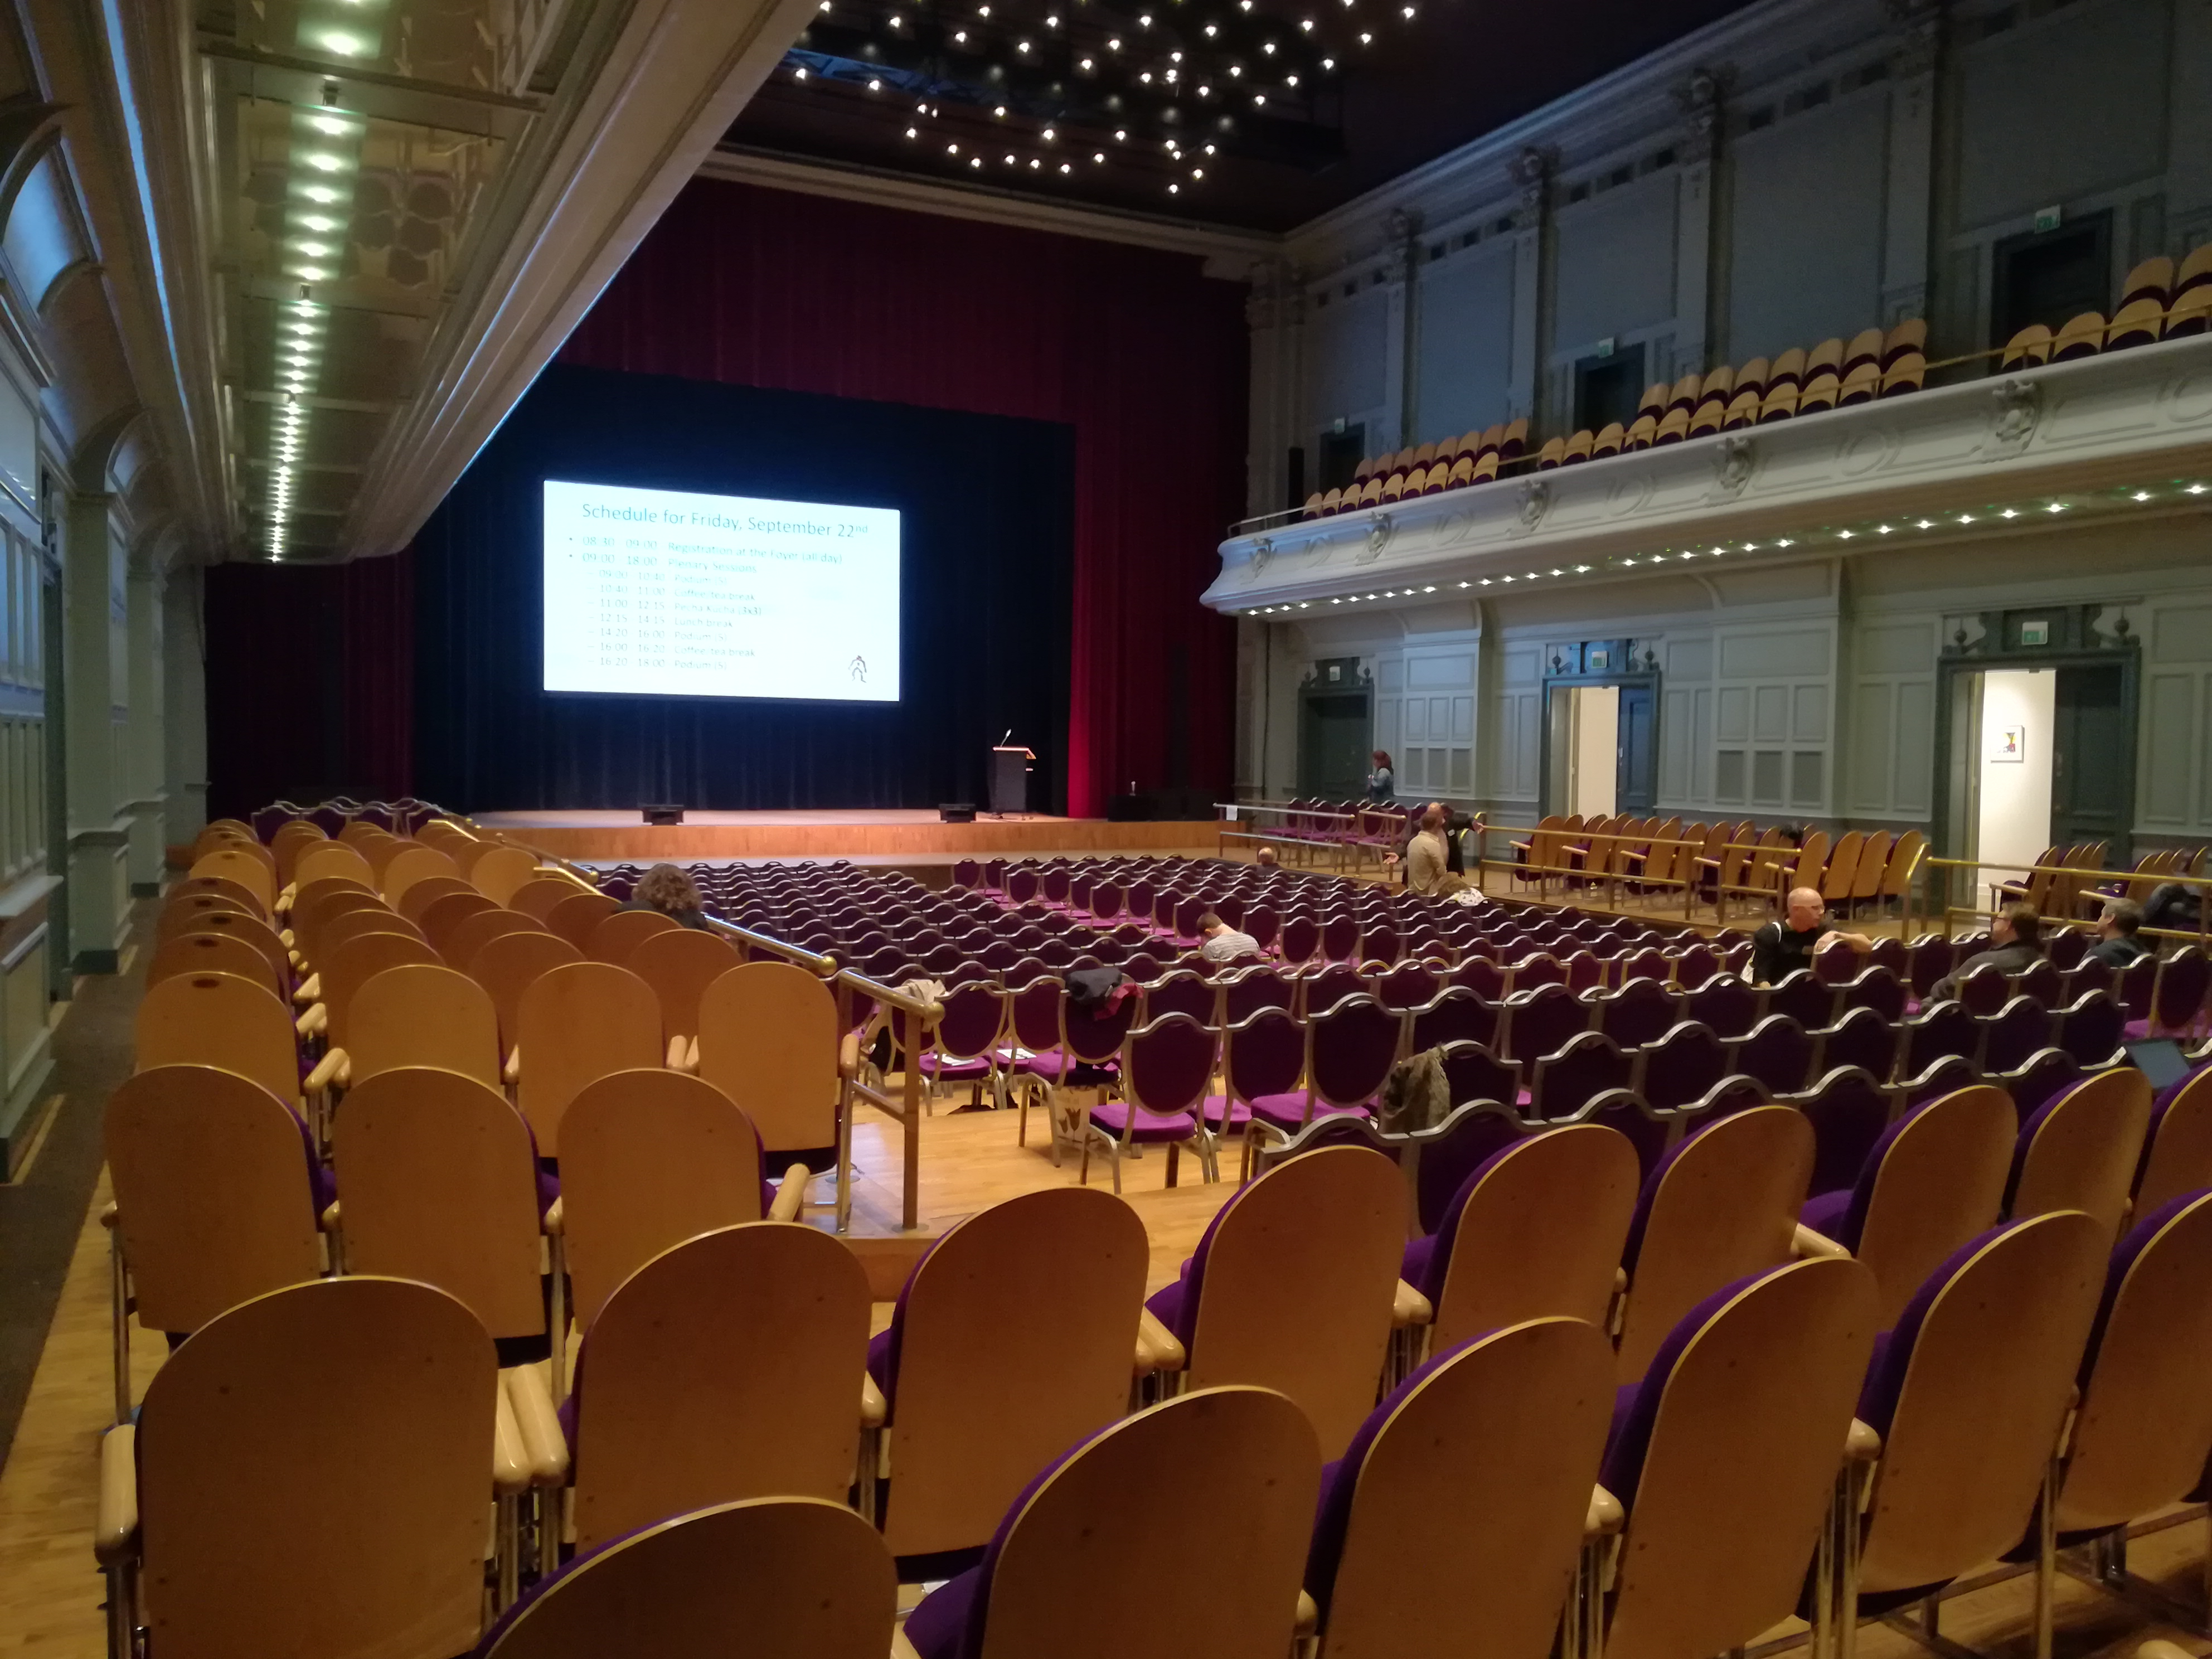
\includegraphics[width=\linewidth]{ESHE_Figure_1}
	\caption{Stadsgehoorzaal lecture hall, which hosted the Podium and Pecha Kucha presentations given at the ESHE
		{\normalfont\scriptsize \\ \copyright\ by
			\shortauthor
			Picture taken by the author.
	}}
	\label{fig:ESHE_Figure_1}
\end{figure}

On the evening of the 20th of September, there was a public lecture at the Rijksmuseum van Oudheden, by Dr. Marie Soressi on the topic of ‘Neanderthals and us: news from our ancestors, and why it matters’. She explored recent ground-breaking developments in ancient DNA studies and how they provide information on the genetic histories of present populations, and the significance of Neanderthal interactions with modern humans in Europe.

Throughout the conference, the ESHE explored ‘classic’ themes, such as palaeoanthropological research, such as the study of new dental remains from Atapuerca-TD6 by María Martinón-Torres, a comparative assessment of premolar root and canal variation in the hominin clade by Matthew Skinner, or the highly-visual presentation on trabecular bone patterning across the human hand among past and present populations by Nicholas Stephens (\cref{fig:ESHE_Figure_2}).

%FIGURE 2: Nick Stephens podium
\begin{figure}[!htb]
	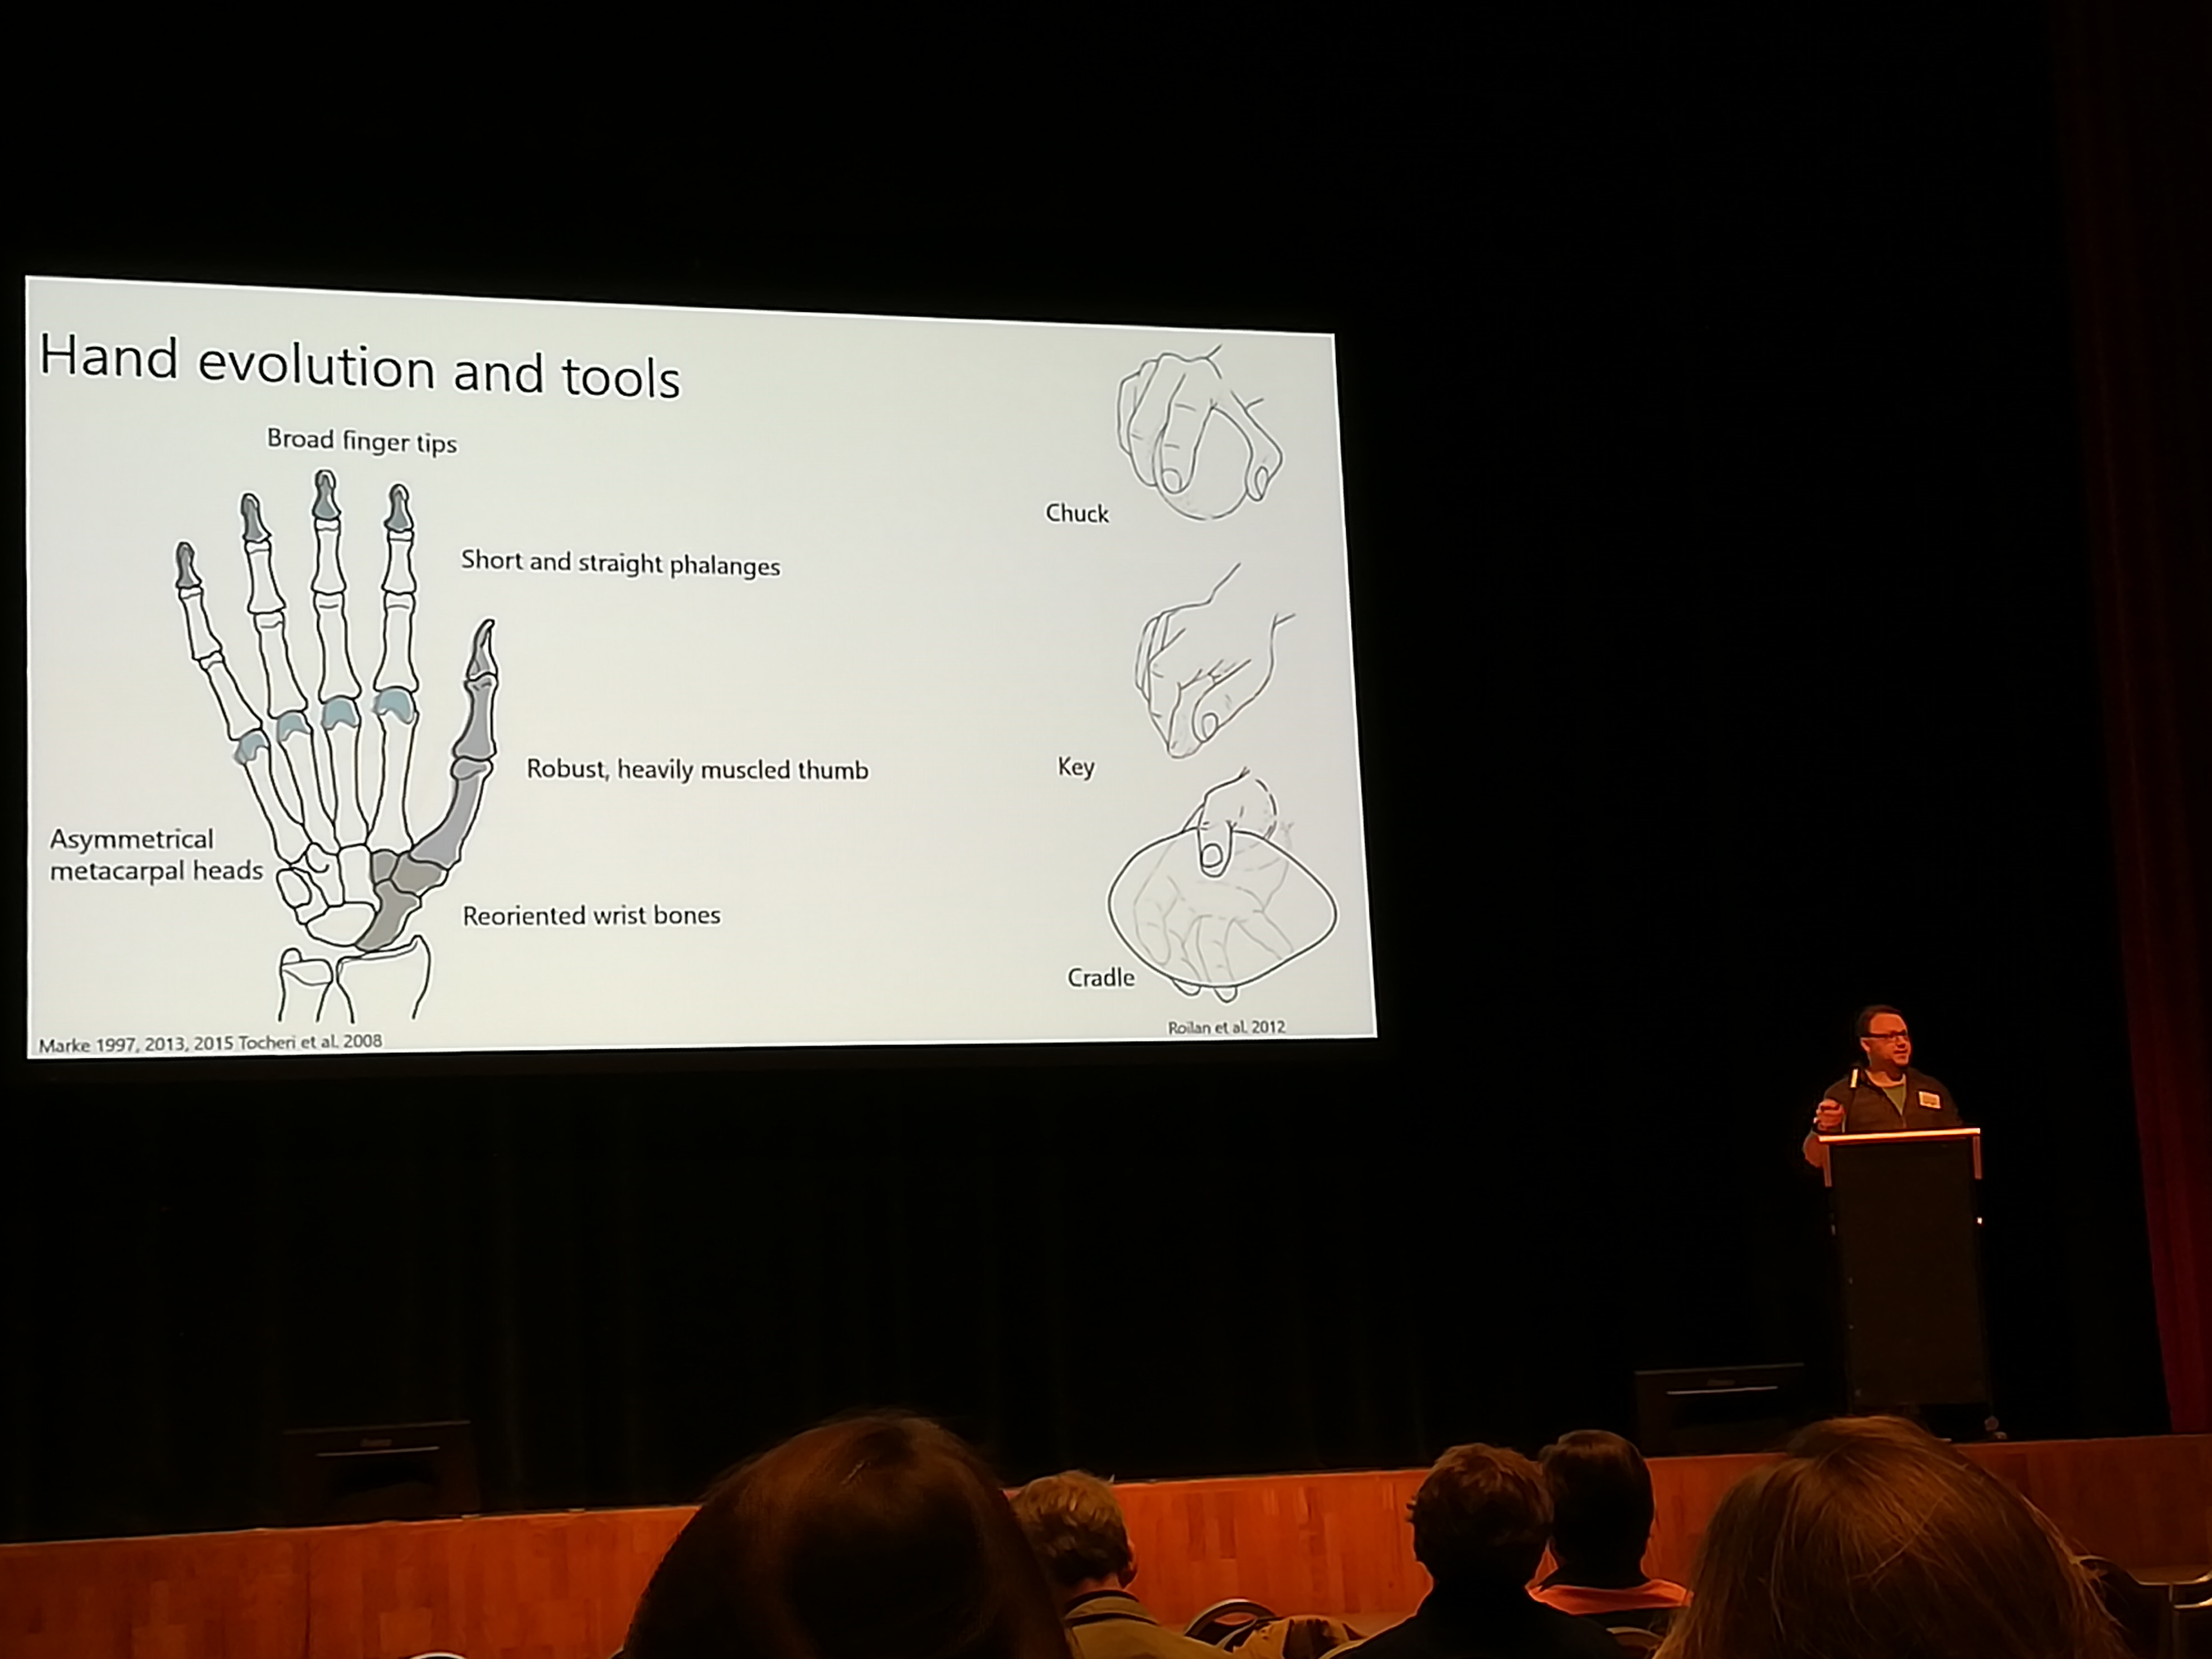
\includegraphics[width=\linewidth]{ESHE_Figure_2}
	\caption{Nick Stephens (MPI-Leipzig) podium presentation on trabecular bone patterning across the human hand
		{\normalfont\scriptsize \\ \copyright\ by
			\shortauthor
			Picture taken by the author, with permission from the presenter.
	}}
	\label{fig:ESHE_Figure_2}
\end{figure}

ESHE also proved to be an unrivalled opportunity to introduce new and promising research projects, such as the excavations at the Middle Pleistocene site of Marathousa I (Greece), directed by Katerina Harvati (Tübingen University), which echoed the excellent preservation at Schöningen. A multidisciplinary team led by Susana Carvalho (University of Oxford) is also starting a long-term project at Gorongosa National Park in Mozambique, the southernmost end of the Rift Valley, which will undoubtedly contribute to better understanding the prehistory of the African continent. Tamara Dogandzic and her team at the Max Planck Institute (MPI-Leipzig) are shedding new light into the Middle-Upper Palaeolithic transition in a key region such as the Balkans. Katerina Douka (Max Planck Institute-Jena) is spearheading a new and game-changing project that innovatively applies ZooMS (Zooarchaeology by Mass Spectrometry) to identify hominin remains in Southern and South-East Asia.

Similarly, several presentations explored alternative perspectives for understanding hominin subsistence practices and lifestyle. These included Amanda Henry’s authoritative reminder of the importance of wild plant foods, particularly tubers and other underground storage organs (USOs), which tend to be available year-round, for understanding winter subsistence by hominin populations, especially in mid and high latitudes. Also in relation to subsistence strategies and their impact in hominin lifestyles, Manuel Will argues that coastal adaptations constitute a “consistent behavioural signature” for Middle Pleistocene hominins, complementing inland resources and thus maximising their “dietary breath and quality”. Lastly, in a highly original piece of research that was awarded the Student Presentation Prize, Andrew Sorensen (Leiden University) explored the potential of handaxes, the multi-purpose tool par excellence, to play a role in the process of fire-making, on the basis of microwear suggesting “repeated percussion and/or forceful abrasion with a hard-mineral material”. The hypothesis is plausible, particularly given the inherent properties of flint for spark-generation.

The chronological framework constitutes a fundamental dimension of archaeological research, and multiple papers were devoted to broadening the range of techniques and refinements within the field, from AMS radiocarbon dating in the Zagros Mountains (Lorena Becerra-Valdivia), Luminescence dating in Shanidar Cave (Marine Frouin), and at Sima de las Palomas (Michael Walker), U-series dating of rock art in Cantabria (Dirk Hoffmann), single-amino-acid radiocarbon dating at Vindija (Thibaut Devièse), and dendrochronology (Sahra Talamo). Understanding the temporality of the archaeological sequence is paramount, and changes in the temporal framework do transform the meaning of the archaeological remains themselves. Particularly striking was Gianpiero di Maida’s re-assessment of Fontana Nuova (Sicily), long-believed to be Aurignacian and thus the oldest site of Sicily. His new data suggest an early Holocene temporal adscription instead. 

The poster sessions, arranged thematically, were a fantastic opportunity for students and professionals alike to engage in networking while having lunch, although the sheer number of posters might have prevented some participants from seeing them all. Of particular interest to me were those related to taphonomy, which explored site formation processes (Domenico Giusti and George Konidaris for Marathousa I, Marta Pernas-Hernández for the avian record of Bell Korongo, Olduvai Gorge, and Gonzalo Linares Matás for the late Early Pleistocene site of Cueva Negra), use-wear in experimental bone tools (Giulia Gallo), and the spatio-temporality of accumulation, such as Nohemi Sala’s study of the hominins from Sima de los Huesos, Spain. Taphonomical issues also featured in some podium presentations, such as Ashley Kruger’s study of post-mortem disarticulation patterns of the \emph{Homo naledi} assemblage from the Dinaledi Chamber, or Laurence Dumounchel’s Pecha Kucha talk assessing the fossil \emph{Suidae} record to understand the environment and subsistence strategies of \emph{Australopithecus anamensis} in the Omo-Turkana basin. Taphonomical research will continue to play a paramount role in understanding the ways in which the archaeological record may inform researchers about the lived experiences of past human populations in their socio-ecological contexts.

The closing Q\&A session tackled important issues regarding the accessibility and organisation of ESHE meetings; for example, after a much-applauded proposal from the audience, the Board promised exploring the viability of childcare provision for future ESHE Conferences.

On the Sunday after the Conference, the local organisers arranged an exclusive guided visit to the Dubois/Trinil collection, housed at the Naturalis Biodiversity Centre, which is currently closed to the public due to ongoing restorations. The exhibition showcased the \emph{‘Pithecanthropus’ erectus} femur, skull cap, and molar (\cref{fig:ESHE_Figure_3_edited}), in addition to the engraved \emph{Pseudodon vondembuschianus trinilensis} shell, the original manuscript in German describing \emph{‘Pithecanthropus’ erectus}. Some fauna from Trinil were also included, such as water buffalo molars (\emph{Bubalus bubalis}); these are interesting to people pursuing zooarchaeological analyses because although their occlusal surfaces resemble those of horses, the roots are more similar to those of other \emph{Artiodactyla}. These guided exhibitions provided attendants with an even more enriching experience.

%FIGURE 3: Homo erectus at Naturalis museum
\begin{figure}[!htb]
	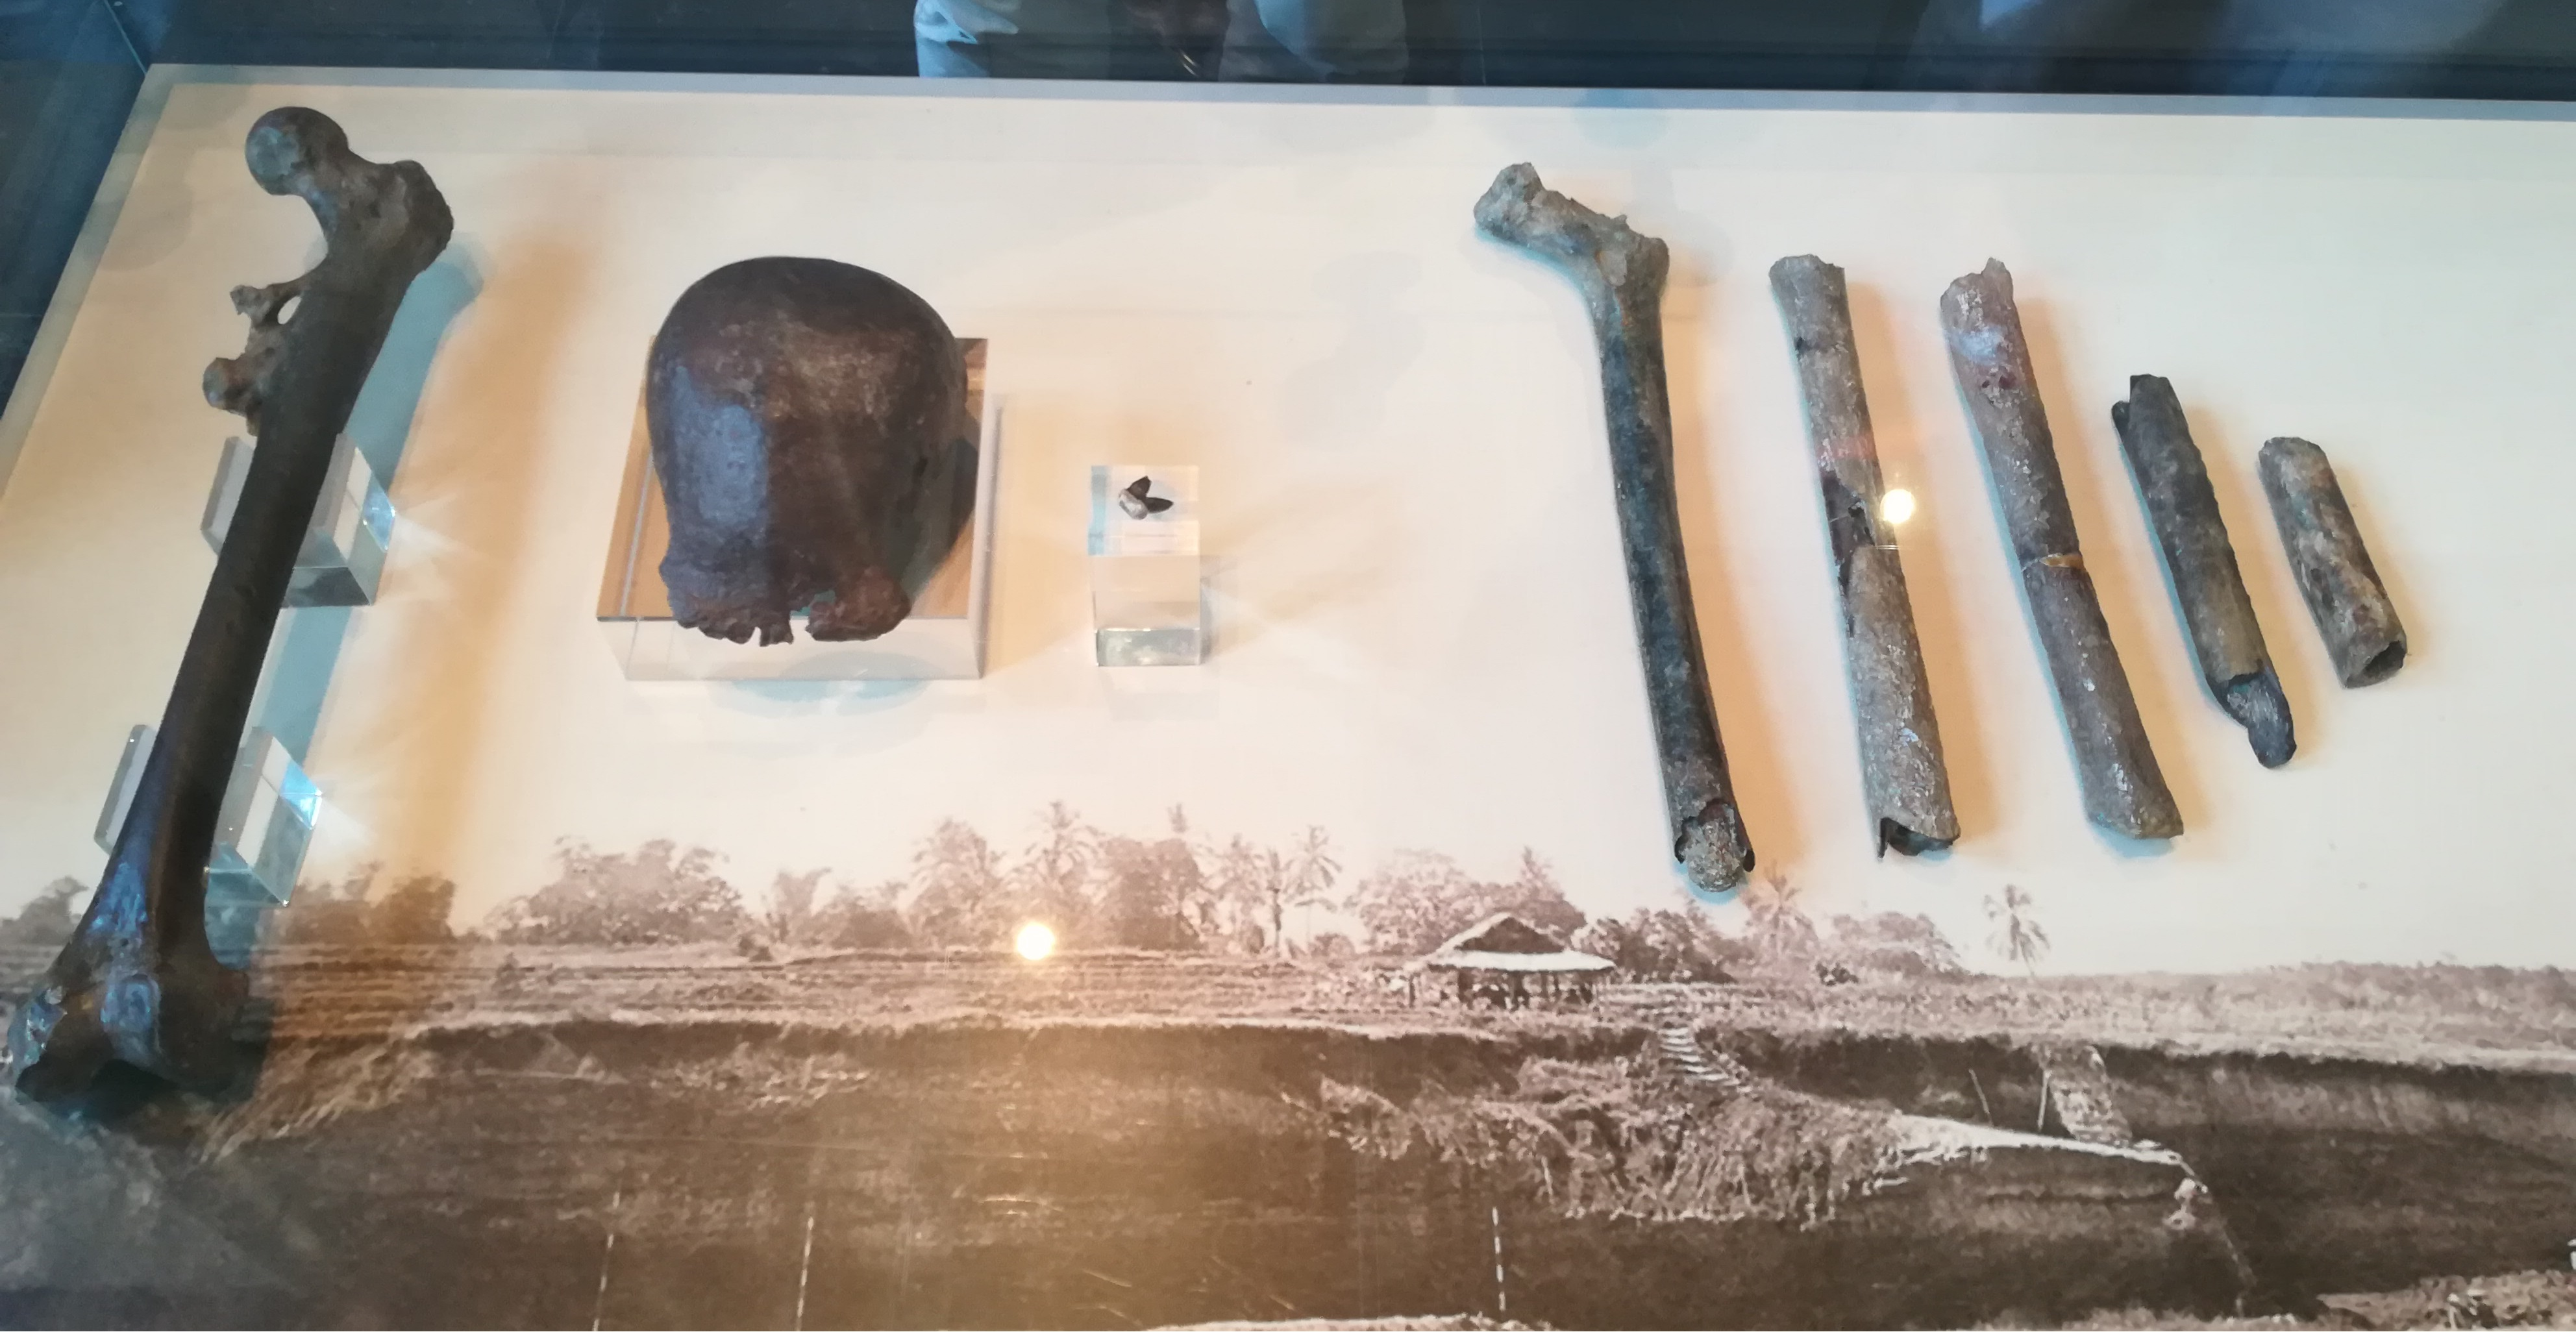
\includegraphics[width=\linewidth]{ESHE_Figure_3_edited}
	\caption{Homo erectus remains from the Dubois-Trinil collection at the Naturalis museum.
		{\normalfont\scriptsize \\ \copyright\ by
			\shortauthor
			Picture taken by the author. With permission from the Naturalis Biodiversity Center.
	}}
	\label{fig:ESHE_Figure_3_edited}
\end{figure}

Overall, the ESHE Conference was a very positive experience, and a great setting for a newcomer to present their first poster at a conference. Next year, the 8\textsuperscript{th} Annual Meeting of the ESHE will be taking place in Faro (Portugal); the sunny beaches of the Algarve seem to be openly promising an enjoyable time learning about human evolution.

\IJSRAclosing%<---- don’t change this!